% ============================================================================
%  CHAPITRE 4 -- CODAGE CONJOINT SOURCE-CANAL APPRIS
% ============================================================================
\chapter{Codage conjoint source-canal appris}
\label{chap:jscc}

Ce chapitre décrit les deux systèmes appris : l'architecture commune, la manière dont le canal entre dans la
boucle d'apprentissage, puis la perte sémantique qui constitue la proposition du projet.

\section{Architecture}
\label{sec:archi_jscc}

Le principe du JSCC profond est de supprimer la frontière entre codage de source et codage de canal. Il n'y a
plus de bits : l'encodeur produit directement les symboles émis.

\paragraph{Encodeur.} Un réseau convolutif réduit l'image d'un facteur 4 en largeur et en hauteur
(deux convolutions de stride 2, suivies de deux blocs résiduels) et produit un tenseur latent
$z \in \mathbb{R}^{16 \times H/4 \times W/4}$. Les activations sont des PReLU.

\paragraph{Couche de canal.} Les valeurs latentes sont tronquées à $c$ canaux, normalisées en puissance, puis
bruitées selon le modèle choisi. Cette opération est \emph{différentiable} : le bruit traverse la
rétropropagation, de sorte que l'encodeur apprend un code adapté au canal plutôt qu'un code optimal en
l'absence de bruit.

\paragraph{Décodeur.} Un réseau symétrique — deux blocs résiduels puis deux convolutions transposées — remonte
à la résolution d'origine, avec une sigmoïde en sortie qui contraint l'image reconstruite dans $[0,1]$.

Le modèle complet compte \num{421715} paramètres. Les deux systèmes appris, syntaxique et sémantique,
partagent \emph{exactement} cette architecture ; leurs fichiers de poids ont la même taille et le même nombre
de paramètres. C'est l'exigence E6 du tableau~\ref{tab:exigences}.

\section{Protocole d'entraînement}
\label{sec:entrainement}

Tous les modèles sont entraînés sur les \num{50000} images d'apprentissage de CIFAR-10~\cite{krizhevsky2009},
avec augmentation par retournement horizontal et recadrage aléatoire, optimiseur Adam et pas d'apprentissage
$10^{-3}$.

Deux tirages aléatoires sont faits à chaque lot :

\begin{itemize}
  \item le \textbf{SNR}, uniformément dans $[0,20]$~dB, pour qu'un seul modèle couvre toute la plage
        d'exploitation ;
  \item le \textbf{nombre de canaux actifs} $c$ parmi $\{2,4,8,12,16\}$, pour l'agilité en bande.
\end{itemize}

Le tableau~\ref{tab:modeles} donne la liste des neuf modèles entraînés et leur coût.

\begin{table}[H]
\centering
\caption{Les neuf modèles entraînés (temps mesurés sur GPU)}
\label{tab:modeles}
\small
\begin{tabularx}{\textwidth}{@{}lrrr>{\raggedright\arraybackslash}X@{}}
\toprule
\textbf{Modèle} & \textbf{Époques} & \textbf{Paramètres} & \textbf{Durée (s)} & \textbf{Rôle} \\
\midrule
\srcfile{clsA}          & 10 & \num{298506} & \num{2296} & classifieur de la perte sémantique \\
\srcfile{clsB}          & 15 & \num{308394} & \num{3388} & juge indépendant \\
\srcfile{dae}           & 25 & \num{421715} & \num{7116} & codeur de source de la chaîne séparée \\
\srcfile{jscc_mse}      & 25 & \num{421715} & \num{8087} & JSCC syntaxique \\
\srcfile{jscc_sem}      & 25 & \num{421715} & \num{1346} & JSCC sémantique (proposition) \\
\srcfile{jscc_mse_snr0} & 15 & \num{421715} & \num{323}  & étude de désadaptation \\
\srcfile{jscc_mse_snr10}& 15 & \num{421715} & \num{349}  & étude de désadaptation \\
\srcfile{jscc_mse_snr20}& 15 & \num{421715} & \num{353}  & étude de désadaptation \\
\srcfile{task}          & 20 & \num{474266} & \num{370}  & extension orientée tâche \\
\bottomrule
\end{tabularx}
\end{table}

\begin{figure}[H]
  \centering
  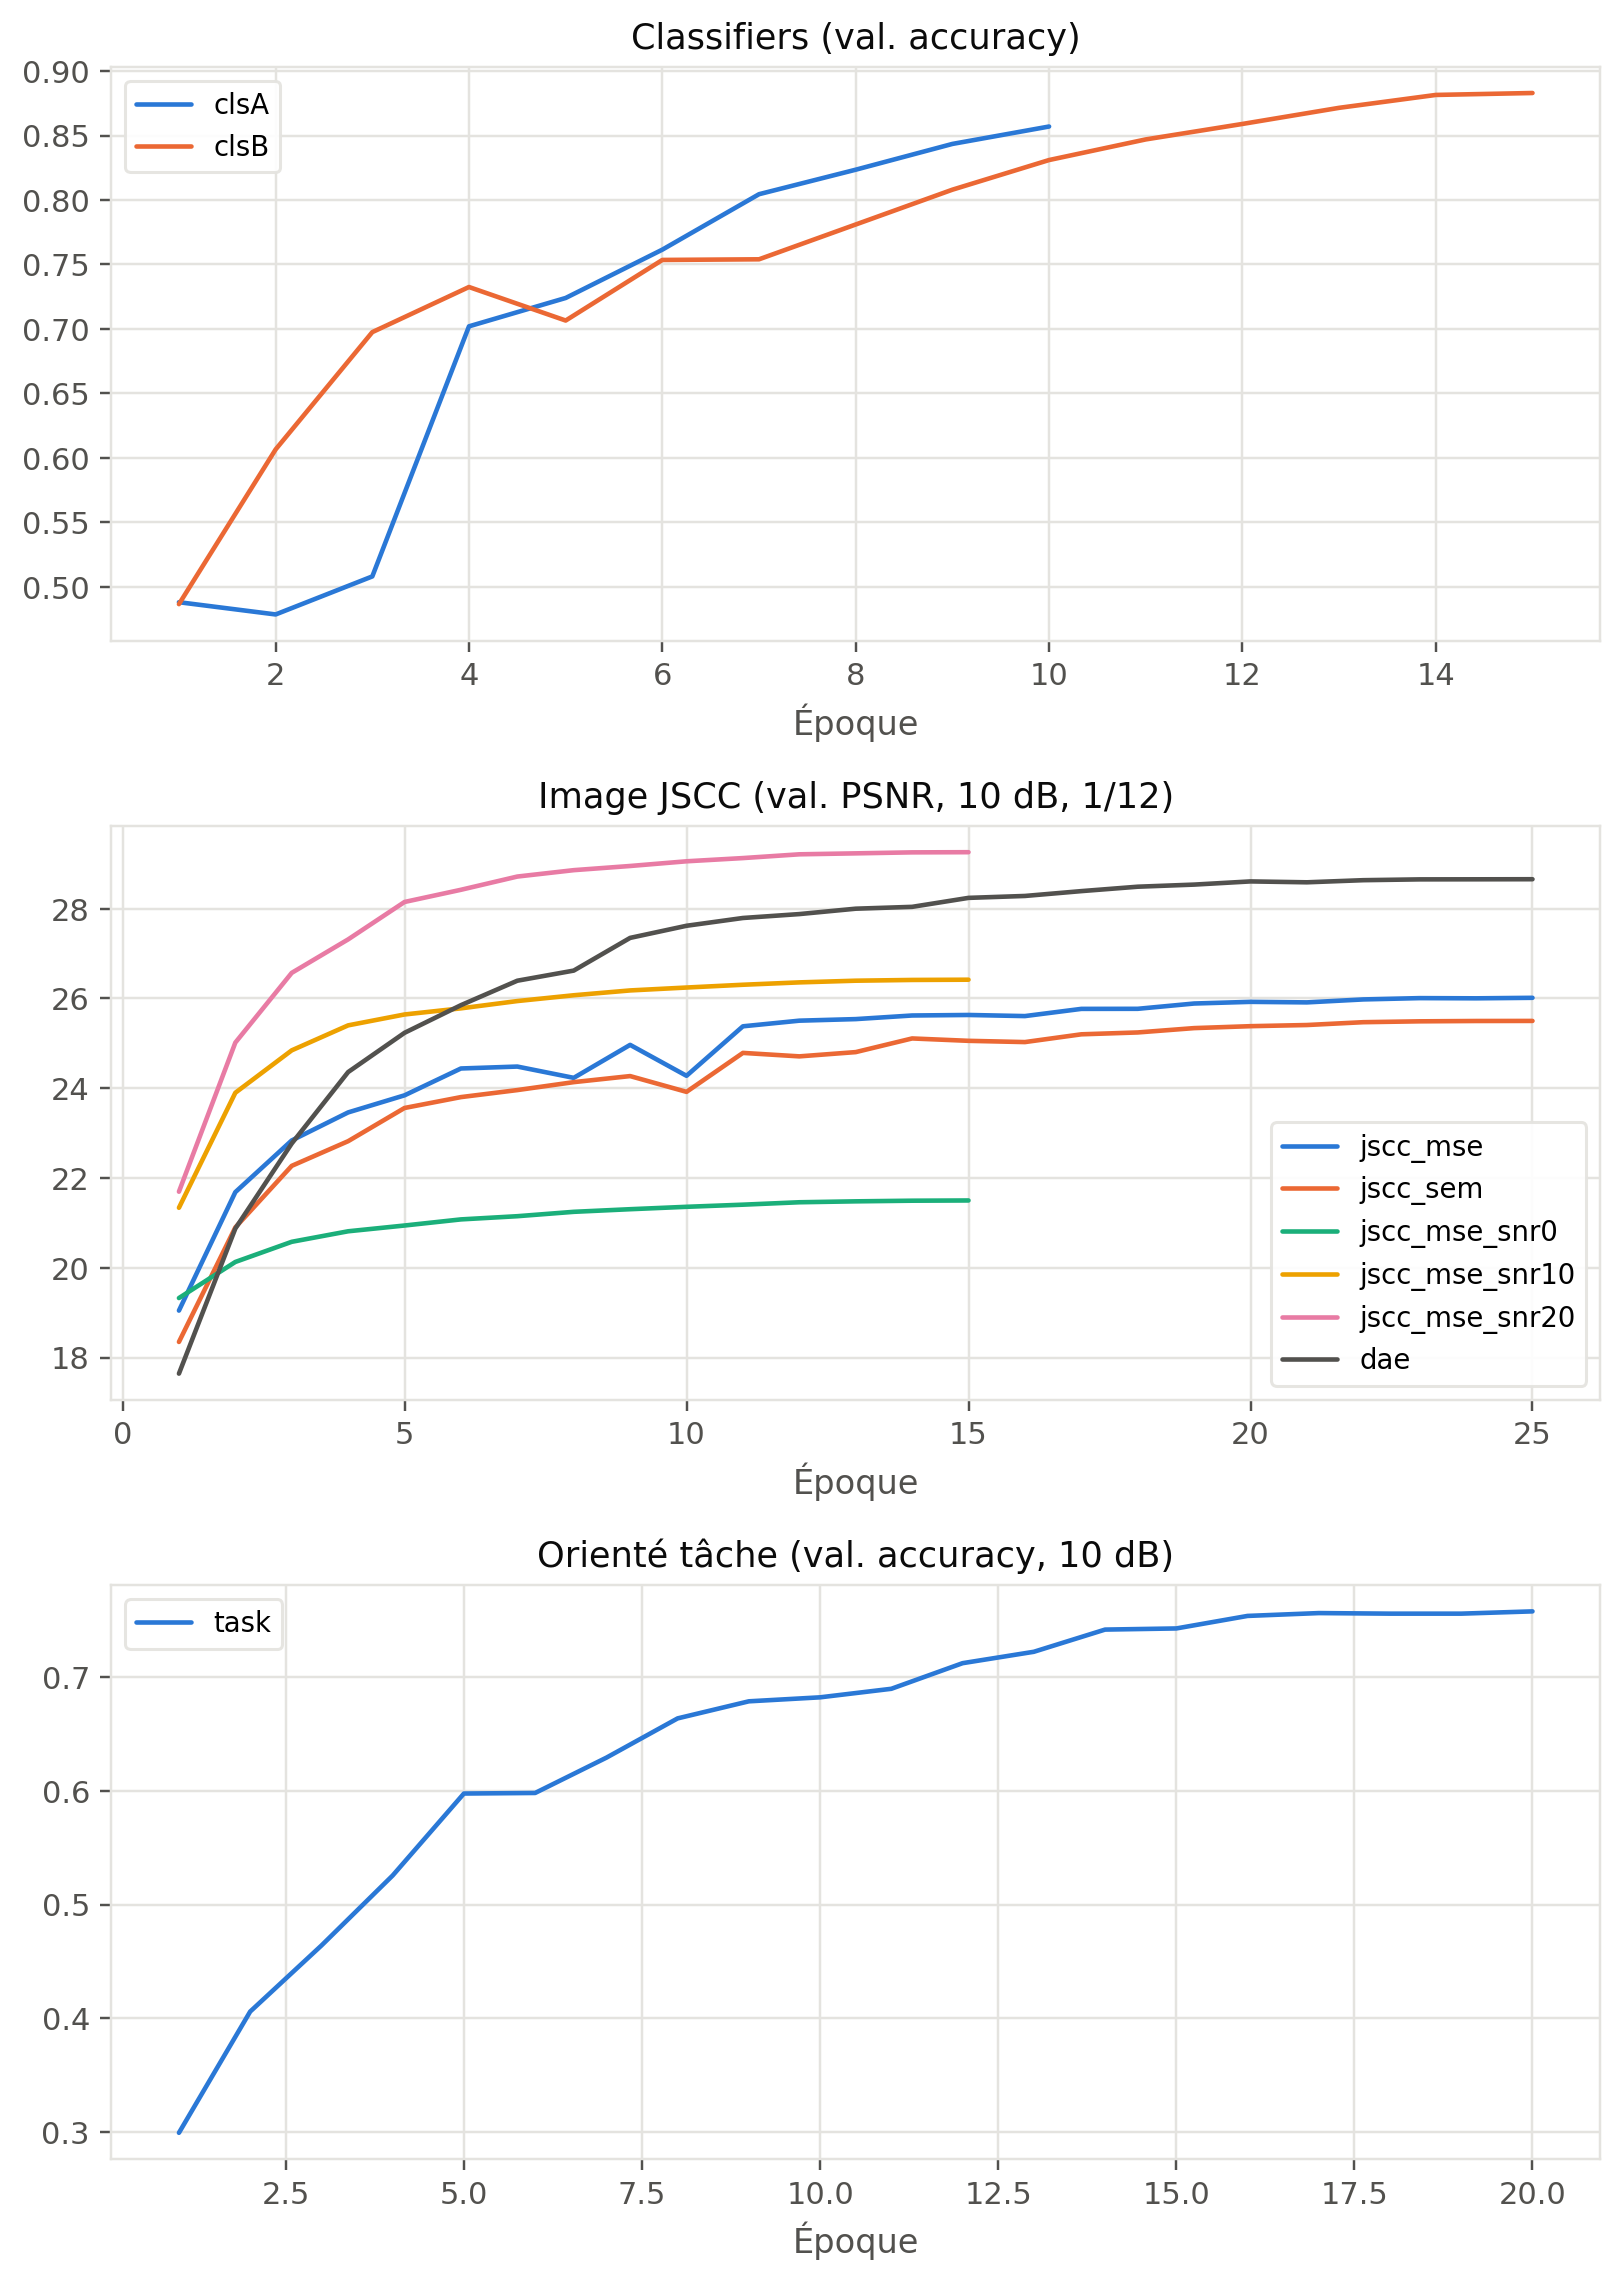
\includegraphics[width=0.78\linewidth]{learning_curves.png}
  \caption{Courbes d'apprentissage des principaux modèles : perte d'entraînement et métrique de validation.}
  \label{fig:learning}
\end{figure}

\section{Système syntaxique : la perte pixel}
\label{sec:jscc_mse}

Le premier système apprend à minimiser l'erreur quadratique moyenne entre l'image reçue et l'originale :
\begin{equation}
  \mathcal{L}_{\text{syn}} = \mathrm{MSE}(\hat{x}, x) .
  \label{eq:loss_mse}
\end{equation}
C'est la formulation de référence de la littérature~\cite{bourtsoulatze2019}. Elle demande des pixels justes,
et rien d'autre.

\section{Système sémantique : la proposition}
\label{sec:jscc_sem}

Le second système ne change \emph{que} la fonction de perte :
\begin{equation}
  \mathcal{L}_{\text{sem}} = \underbrace{\mathrm{MSE}(\hat{x},x)}_{\text{fidélité}}
  \;+\; \lambda_f \underbrace{\mathcal{L}_{\text{feat}}(\hat{x},x)}_{\text{caractéristiques}}
  \;+\; \lambda_t \underbrace{\mathrm{CE}\big(f_A(\hat{x}), y\big)}_{\text{tâche}},
  \qquad \lambda_f = 0{,}01,\; \lambda_t = 0{,}003 .
  \label{eq:loss_sem}
\end{equation}

\paragraph{Terme de caractéristiques.} Il compare les activations internes d'un classifieur $f_A$ \textbf{gelé}
pour l'image reçue et pour l'originale, normalisées par l'énergie de la carte de référence :
\begin{equation}
  \mathcal{L}_{\text{feat}}(\hat{x},x) = \frac{1}{L}\sum_{\ell=1}^{L}
  \frac{\mathrm{MSE}\big(f_A^{(\ell)}(\hat{x}),\, f_A^{(\ell)}(x)\big)}
       {\mathbb{E}\big[f_A^{(\ell)}(x)^2\big]} .
  \label{eq:loss_feat}
\end{equation}
C'est une perte perceptuelle au sens de Johnson \emph{et al.}~\cite{johnson2016} : elle demande que l'image
reste la même \emph{vue par un réseau}, et non pixel par pixel.

\paragraph{Terme de tâche.} L'entropie croisée entre la prédiction du classifieur gelé sur l'image reçue et
l'étiquette vraie. Il demande simplement que la classe reste décodable après transmission.

\paragraph{Pondération.} Les coefficients sont faibles — $1\%$ et $0{,}3\%$ — et ce choix est délibéré : le
sens est un \emph{ajout} à la fidélité, pas un remplacement. Une pondération plus forte produirait des images
flatteuses pour le classifieur mais visuellement dégradées, ce qui déplacerait le compromis au lieu de
l'améliorer.

\begin{keybox}[Pourquoi le classifieur est gelé]
$f_A$ n'est pas entraîné pendant l'optimisation du JSCC : ses poids sont figés et seuls les gradients le
traversent. S'il était entraîné conjointement, il lui suffirait de s'adapter aux artefacts du décodeur pour
faire baisser la perte sans que le sens soit mieux transmis. Le gel est donc une condition de validité, pas un
détail d'implémentation.
\end{keybox}

\section{Comparaison des signaux émis}
\label{sec:signaux}

La différence la plus visible entre les deux familles de systèmes apparaît dans le plan complexe. La chaîne
numérique émet des points discrets et réguliers — une constellation — et le bruit fait franchir des frontières
de décision, ce qui produit des bits faux. Le JSCC émet un \emph{nuage continu} : il n'y a pas de frontière à
franchir, donc pas de seuil, et le bruit se traduit par une dégradation graduelle de la reconstruction. C'est
l'explication directe de la disparition de l'effet falaise, que le chapitre~\ref{chap:resultats} quantifie et
que le simulateur du chapitre~\ref{chap:simulateur} donne à voir directement.
